\documentclass[conference]{IEEEtran}

\usepackage{fontspec}
\usepackage{xeCJK}
\setmainfont{Times New Roman}
\setCJKmainfont{FandolSong-Regular}
\setCJKsansfont{FandolHei-Regular}
\usepackage{amsmath,amssymb}
\usepackage{graphicx}
\usepackage{booktabs}
\usepackage{array}
\usepackage{float}
\usepackage{cite}
\usepackage{url}
\usepackage[hidelinks]{hyperref}

\newcommand{\method}{预算协同检索}
\newcommand{\eg}{e.g.}

\title{面向低算力机械故障辅助诊断的预算约束型向量与图协同证据检索方法\\
\large Budget-Constrained Vector-Graph Collaborative Evidence Retrieval for Compute-Efficient Mechanical Fault Diagnosis}

\author{
\IEEEauthorblockN{张晓坤\textsuperscript{1}，符栋梁\textsuperscript{1}，王睿\textsuperscript{2,*}}
\IEEEauthorblockA{\textsuperscript{1}中国船舶集团有限公司第七〇四研究所，上海，中国}
\IEEEauthorblockA{\textsuperscript{2}同济大学电子与信息工程学院，上海，中国\\
\textsuperscript{*}通信作者：王睿（\href{mailto:ruiwang@tongji.edu.cn}{ruiwang@tongji.edu.cn}）}}

\begin{document}
\maketitle

\begin{abstract}
面向船舶机舱等低算力部署场景，本地小规模大语言模型容易受到无关证据、冗余上下文和多次验证调用的影响。普通稠密检索虽然能够扩大召回范围，但在固定证据预算内仍可能混入与诊断任务不一致、故障对象不匹配或来源重复的内容，增加模型推理负担。本文提出一种预算约束型向量与图协同证据检索方法。该方法先利用BGE-M3进行宽召回，再结合诊断任务约束、故障对象约束、一跳图传播和来源去冗余，在最大预算$K=3$内选择紧凑证据集；候选不足时不强制填满预算。本地Qwen2.5-7B仅对入选证据进行二进制支持性核验，最终由确定性渲染器输出带证据编号的辅助诊断建议或明确拒答。高可信三元组图谱在系统中仅作为离线证据底座，其作用是提供原文锚点和局部结构。在40条机械故障诊断查询上，本文方法相对稠密检索将Recall由0.218提高到0.431，NDCG由0.406提高到0.822，引用F1由0.259提高到0.426；平均提示长度由1066.7降至634.7 Token，模型调用次数由2.95降至1.80，平均端到端时延由839.4 ms降至531.2 ms。回答原子陈述的严格证据支持率达到91.0\%，所有可回答问题均得到有效回答，所有不可回答问题均被正确拒答。结果表明，该方法能够在不扩大模型规模的情况下减少推理负担，提高回答的证据一致性，并为低算力机械故障辅助诊断提供低时延、可核验的建议。
\end{abstract}

\begin{IEEEkeywords}
机械故障辅助诊断，证据预算，向量与图协同检索，低算力推理，检索增强生成，本地大语言模型
\end{IEEEkeywords}

\section{引言}

船舶机舱泵系故障辅助诊断要求模型在有限时间内给出有依据的症状解释、原因分析、检查方法或维护建议。检索增强生成（Retrieval-Augmented Generation，RAG）可为大语言模型提供外部知识\cite{lewis2020rag}，但“检索更多证据”并不必然带来更好的回答。对于本地7B模型，无关或重复证据会占用上下文窗口，并增加证据核验次数。推理时延随提示长度和模型调用数上升，低算力部署尤其容易受到影响。

稠密检索擅长语义宽召回，却难以稳定区分症状、原因、检查和维护等诊断任务。图检索能够利用实体关系补充结构信息\cite{edge2024graphrag,sun2024think,he2024gretriever,zhu2025kg2rag}，但如果不控制进入模型的证据数量，图扩展同样会产生额外上下文。本文关注的核心问题是：在模型规模和最大证据数均固定时，如何利用向量相关性与局部图结构选择少量有效证据，使回答质量提高的同时降低推理负担和端到端时延。

本文的贡献集中在在线检索与推理协同。主要贡献如下：

\begin{itemize}
    \item 提出预算约束型向量与图协同证据检索方法。方法将稠密相关性、诊断任务约束、故障对象亲和度、一跳图接近度和来源去冗余统一到最大预算$K=3$的选择过程，并允许主动欠填。
    \item 面向本地7B模型建立“少量证据选择--二进制支持核验--确定性回答”的推理流程。该流程避免自由生成引入的额外不确定性，并通过缩短提示和减少调用降低模型负担。
    \item 在同模型、同证据预算条件下进行质量与时延联合评价。结果同时覆盖检索质量、引用准确性、回答与拒答行为、提示长度、模型调用和端到端时延，并通过配对统计检验验证主要改进。
\end{itemize}

\section{相关工作}

BGE-M3支持多语言和多粒度文本表示\cite{chen2024bgem3}，适合工业技术文档的稠密召回。Qwen2.5提供开放权重的多规模指令模型\cite{yang2024qwen}。本文固定使用Qwen2.5-7B，不通过扩大模型规模或微调获取增益。与通过改写提示减少Token的压缩方法\cite{jiang2023llmlingua}不同，本文保留原始证据文本，在检索端控制证据数量和验证次数。

GraphRAG及相关方法通过图搜索、相关子图或知识图谱引导检索\cite{edge2024graphrag,sun2024think,he2024gretriever,zhu2025kg2rag}。本文不执行深层开放路径推理，而将一跳图传播作为固定预算内的候选补充信号。ALCE\cite{gao2023alce}和RAGAs\cite{es2024ragas}强调引用正确性、检索相关性和回答忠实性。选择性问答与Self-RAG进一步说明，可靠拒答和自检是可信问答的重要组成部分\cite{kamath2020selective,asai2024selfrag}。本文据此同时评价证据选择、引用支持、拒答和推理代价。

\begin{figure*}[!t]
    \centering
    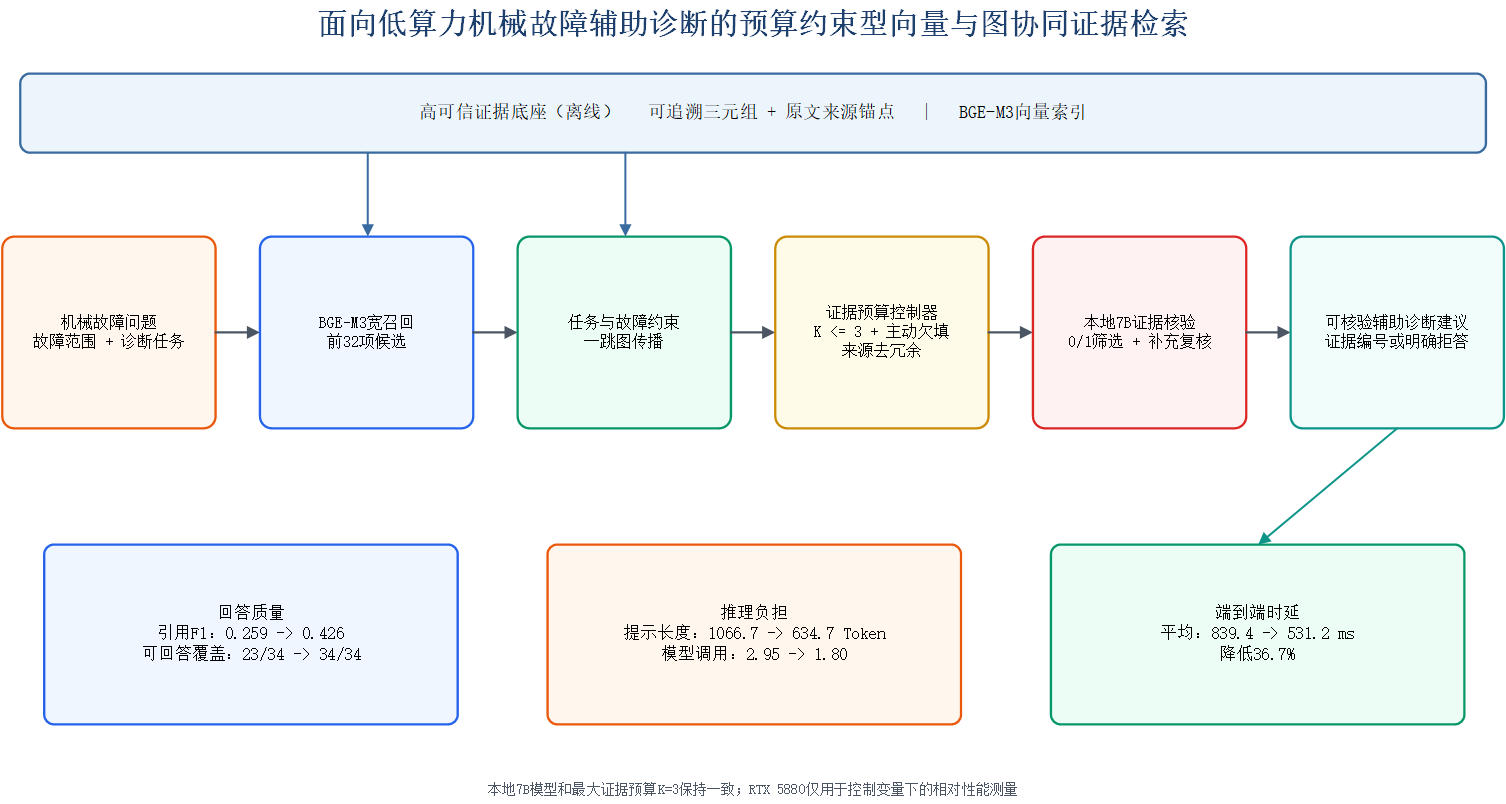
\includegraphics[width=0.98\textwidth]{figures/rp2_budgeted_retrieval_zh.png}
    \caption{预算约束型向量与图协同证据检索流程。方法在固定本地7B模型下压缩无效证据和验证工作量，并输出可核验建议或明确拒答。}
    \label{fig:pipeline}
\end{figure*}

\section{预算约束型向量与图协同检索}

\subsection{问题定义与推理负担}

查询表示为$q=(x,f,r)$，其中$x$为自然语言问题，$f$为目标故障范围，$r$为症状、原因或机理、检查、维护中的一种诊断任务。离线证据底座提供规范化三元组、原文证据、来源锚点和BGE-M3向量索引。其构建方法属于前序研究，本文只使用固定发布版本。

对本地模型而言，在线推理负担主要由累计提示长度$T_{\mathrm{prompt}}$和模型调用次数$N_{\mathrm{call}}$决定。本文将其表示为

\begin{equation}
L_{\mathrm{inf}}(q)=\alpha T_{\mathrm{prompt}}(q)+\beta N_{\mathrm{call}}(q),
\label{eq:load}
\end{equation}

其中$\alpha$与$\beta$由具体硬件和推理框架决定。本文不直接拟合二者，而是分别测量提示长度、调用次数和端到端时延。证据预算是连接检索质量与推理负担的控制变量。

\subsection{宽召回、结构约束与预算选择}

BGE-M3首先返回前32项候选，并以前8项证据的端点实体作为图锚点。锚点分数沿实体邻接关系传播一跳，衰减系数为0.70。候选证据$e$的基础分数为

\begin{equation}
b(e,q)=s_d(e,q)+0.24s_g(e,q)+0.10c(e)+0.35a(e,q),
\label{eq:base}
\end{equation}

其中$s_d$为稠密相似度，$s_g$为一跳图接近度，$c(e)$为证据置信先验，$a(e,q)$为故障名称与证据端点的字符二元组Dice相似度。诊断任务约束优先保留与问题类型一致的证据，故障对象约束删除明显错配的内容。

系统采用以下边际增益进行贪心选择：

\begin{equation}
\Delta(e\mid S,q)=b(e,q)+0.06\,\mathbb{I}[\phi(e)\notin\Phi(S)],
\label{eq:select}
\end{equation}

$\phi(e)$表示证据的来源族，第二项用于降低同源重复。选择过程满足$|S|\leq K$，本文固定$K=3$。$K$是上限而非固定输入数。候选不满足任务或故障约束时，系统不强制填满，从源头减少无效上下文。

\subsection{本地7B证据核验与确定性回答}

Qwen2.5-7B不直接自由生成完整诊断文本。第一阶段只对候选输出等长0/1支持掩码；第二阶段对首轮未通过的候选逐条进行召回导向复核，输出仍限制为0或1。非法格式、长度不一致和非二进制结果均按不支持处理。通过核验的证据由确定性渲染器转换为原子回答点，并附证据编号。没有合格证据时，系统明确输出证据不足。

图\ref{fig:pipeline}展示了完整流程。离线图谱只向在线检索提供可信证据和一跳结构。本文方法的重点是中间的约束选择、预算控制和本地模型核验。

\section{实验设计}

\subsection{数据与对照方法}

受控开发集由10类泵系故障与4类诊断任务组合成40条查询，其中34条可由固定证据图谱回答，6条用于检验拒答。在线系统只能读取自然语言问题、故障范围、诊断任务及公开证据字段，不得访问基准相关性标签。另构造80条未参与参数选择的确定性改写问题，用于检验措辞变化下的稳定性。四份独立外部文档仅在协议固定后用于一次描述性检查，不回流调整参数。

所有主方法采用相同的最大预算$K=3$。对照包括：（1）仅使用稠密相似度的“稠密检索”；（2）加入诊断任务约束的“稠密+任务”；（3）进一步加入一跳传播的“稠密+任务+图”；（4）加入故障对象约束、来源去冗余、主动欠填和两阶段7B核验的本文方法。另设置“本文方法（去图）”，只关闭图传播，用于观察图结构的边际作用。

\subsection{指标与运行环境}

质量指标包括Recall、NDCG和引用Precision、Recall、F1。回答行为指标包括可回答问题覆盖率、不可回答问题拒答率和原子陈述严格支持率。效率指标包括提示Token数、模型调用次数、检索时延、核验时延和端到端时延。主要差异采用按故障类别成簇的5000次配对Bootstrap，报告95\%置信区间。

系统面向低算力部署，但为保证各方法处于相同且稳定的运行状态，实验统一在NVIDIA RTX 5880 Ada 48 GB上进行。Qwen2.5-7B以BF16完整加载到单GPU，不发生CPU或磁盘卸载。时延包含检索、提示构造、证据核验和回答渲染，不包含模型加载、索引构建与预热。因此，实验结论针对同硬件下的相对质量与效率，不把RTX 5880视为低算力设备。

\section{实验结果}

\subsection{回答质量与端到端效率}

表\ref{tab:main}给出相同最大证据预算下的主结果。本文方法相对稠密检索将Recall提高0.2127，NDCG提高0.4166，引用F1提高0.1672，平均端到端时延降低308.2 ms。四项差异的95\%置信区间分别为$[0.1496,0.2748]$、$[0.3184,0.4940]$、$[0.1075,0.2298]$和$[-395.3,-217.2]$ ms，均不跨零。质量提升没有依赖更多证据，反而伴随更低的推理成本。

\begin{table}[H]
\centering
\caption{相同最大证据预算$K=3$下的主实验结果}
\label{tab:main}
\setlength{\tabcolsep}{2.5pt}
\resizebox{\columnwidth}{!}{%
\begin{tabular}{lccccc}
\toprule
方法 & Recall & NDCG & 引用P/R/F1 & 作答/拒答R & 均值/p95(ms) \\
\midrule
稠密检索 & 0.218 & 0.406 & 0.574/0.197/0.259 & 0.676/1.000 & 839.4/1113.1 \\
稠密+任务 & 0.378 & 0.678 & 0.721/0.299/0.372 & 0.853/1.000 & 782.1/1109.6 \\
稠密+任务+图 & 0.405 & 0.716 & 0.750/0.302/0.377 & 0.882/1.000 & 805.5/1101.6 \\
\textbf{本文方法} & \textbf{0.431} & \textbf{0.822} & \textbf{0.799/0.370/0.426} & \textbf{1.000/1.000} & \textbf{531.2/892.5} \\
\bottomrule
\end{tabular}
}
\end{table}

本文方法平均保留2.25条证据，提示长度由1066.7降至634.7 Token，模型调用次数由2.95降至1.80。提示长度、调用数和平均端到端时延分别下降40.5\%、39.0\%和36.7\%。这说明时延优势主要来自预算约束和主动欠填，而不是更换更快的模型。

\subsection{图传播、核验器与可信回答}

在检索层，“稠密+任务+图”相对“稠密+任务”的Recall提高0.0268，95\%置信区间为$[0.0031,0.0616]$；NDCG提高0.0381，95\%置信区间为$[0.0059,0.0804]$。图传播能够改善候选召回与排序。完整系统中，去除图传播后的平均指标变化较小，差异未达到统计显著；但图传播补回了一个无图方法遗漏的不对中检查问题，使可回答覆盖由33/34提高到34/34，平均时延仅增加14.2 ms。图模块更适合作为低成本的尾部召回补充，而不是全部性能提升的唯一来源。

两阶段证据核验解决了精确性与覆盖之间的冲突。只使用首阶段筛选时，引用Precision达到0.818，但漏掉一条可回答问题；增加召回复核后，34条可回答问题全部作答，6条不可回答问题全部拒答，引用Precision仍为0.799。自动一致性核验覆盖160条回答和323个原子项。本文方法的原子陈述严格支持率为91.0\%，整段回答严格支持率为82.4\%，所有原子陈述均获支持的回答比例为88.2\%，引文片段原文核验率为100\%。这些指标衡量建议与引用证据的一致性，不等同于实际设备维修决策的最终正确率。

\subsection{措辞稳定性}

在80条未参与参数选择的改写问题上，本文方法取得0.383的Recall和0.737的NDCG，高于“稠密+任务+图”的0.338和0.645。原问题与改写问题的证据集合平均Jaccard相似度为0.742，首位证据一致率为0.725。结果说明方法的排序优势不依赖单一固定句式，但当前实验仍假设故障范围和诊断任务已知。

\section{讨论}

本文方法的核心优势是以检索端预算控制换取推理端收益。稠密宽召回保证候选范围，任务与故障约束减少错配证据，一跳图传播补充结构相关的尾部候选，来源去冗余和主动欠填控制实际输入规模。本地7B只判断证据是否支持问题，确定性渲染器负责形成回答。该分工降低了小模型处理无效上下文和自由生成文本的负担。

高可信证据图谱是本研究的输入基础，而不是主要创新对象。本文所称高可信，是指证据记录通过自动结构约束、原文支持检查和来源完整性检查，并能回溯到原文、页码、网址和哈希。在线研究不再讨论图谱构建细节，只利用其证据锚点和局部邻接关系。论文贡献应归于预算约束型向量与图协同检索及其对本地模型推理负担的控制。

当前实验仍有两项边界。第一，40条查询属于受控机械故障能力测试，故障范围和诊断任务作为系统输入给出，尚未评价开放式意图识别。第二，实验在统一服务器GPU上测量相对效率，尚未在实际船载低功耗设备上验证绝对时延。后续工作将保持算法和模型配置不变，在目标硬件上补充显存、能耗和并发吞吐测试。

\section{结论}

本文提出面向低算力机械故障辅助诊断的预算约束型向量与图协同证据检索方法。方法在最大证据预算$K=3$内联合稠密相关性、诊断任务、故障对象、局部图结构和来源多样性，并通过主动欠填与两阶段支持性核验减少本地7B模型的无效推理。实验显示，该方法同时提高检索与引用质量，降低提示长度、模型调用次数和端到端时延，并能够输出有原文依据的辅助诊断建议或可靠拒答。结果支持在不扩大模型规模的条件下，通过检索预算和结构约束提高机械故障问答的质量与运行效率。

\section*{数据与声明}

\textbf{数据可用性：}固定配置、代码、可追溯证据评价集、聚合结果和结果清单计划通过匿名或公开仓库提供。受版权限制的原始PDF不再分发，证据记录保留来源网址、页码和哈希。

\textbf{伦理、利益冲突：}本研究不涉及人体、动物实验或个人敏感数据。本人声明不存在已知利益冲突。

\textbf{生成式人工智能使用说明：}生成式人工智能用于代码辅助、实验日志整理和语言组织；研究设计、实验执行、统计核验、引用核查和论文最终责任由作者承担。

\IEEEtriggeratref{9}
\begin{thebibliography}{14}

\bibitem{lewis2020rag} P. Lewis et al., ``Retrieval-augmented generation for knowledge-intensive NLP tasks,'' in \emph{Advances in Neural Information Processing Systems}, vol. 33, pp. 9459--9474, 2020.

\bibitem{edge2024graphrag} D. Edge et al., ``From local to global: A Graph RAG approach to query-focused summarization,'' arXiv:2404.16130, 2024, rev. 2025, doi: 10.48550/arXiv.2404.16130.

\bibitem{chen2024bgem3} J. Chen, S. Xiao, P. Zhang, K. Luo, D. Lian, and Z. Liu, ``M3-Embedding: Multi-linguality, multi-functionality, multi-granularity text embeddings through self-knowledge distillation,'' in \emph{Findings of ACL 2024}, pp. 2318--2335, 2024, doi: 10.18653/v1/2024.findings-acl.137.

\bibitem{yang2024qwen} A. Yang et al., ``Qwen2.5 technical report,'' arXiv:2412.15115, 2024, rev. 2025.

\bibitem{sun2024think} J. Sun et al., ``Think-on-Graph: Deep and responsible reasoning of large language model on knowledge graph,'' in \emph{Proc. ICLR}, 2024.

\bibitem{he2024gretriever} X. He et al., ``G-Retriever: Retrieval-augmented generation for textual graph understanding and question answering,'' in \emph{Advances in Neural Information Processing Systems}, vol. 37, 2024, doi: 10.52202/079017-4224.

\bibitem{zhu2025kg2rag} X. Zhu, Y. Xie, Y. Liu, Y. Li, and W. Hu, ``Knowledge graph-guided retrieval augmented generation,'' in \emph{Proc. NAACL-HLT}, vol. 1, pp. 8912--8924, 2025, doi: 10.18653/v1/2025.naacl-long.449.

\bibitem{gao2023alce} T. Gao, H. Yen, J. Yu, and D. Chen, ``Enabling large language models to generate text with citations,'' in \emph{Proc. EMNLP}, pp. 6465--6488, 2023, doi: 10.18653/v1/2023.emnlp-main.398.

\bibitem{es2024ragas} S. Es, J. James, L. Espinosa Anke, and S. Schockaert, ``RAGAs: Automated evaluation of retrieval augmented generation,'' in \emph{Proc. EACL System Demonstrations}, pp. 150--158, 2024, doi: 10.18653/v1/2024.eacl-demo.16.

\bibitem{kamath2020selective} A. Kamath, R. Jia, and P. Liang, ``Selective question answering under domain shift,'' in \emph{Proc. ACL}, pp. 5684--5696, 2020, doi: 10.18653/v1/2020.acl-main.503.

\bibitem{asai2024selfrag} A. Asai, Z. Wu, Y. Wang, A. Sil, and H. Hajishirzi, ``Self-RAG: Learning to retrieve, generate, and critique through self-reflection,'' in \emph{Proc. ICLR}, 2024.

\bibitem{jiang2023llmlingua} H. Jiang, Q. Wu, C.-Y. Lin, Y. Yang, and L. Qiu, ``LLMLingua: Compressing prompts for accelerated inference of large language models,'' in \emph{Proc. EMNLP}, pp. 13358--13376, 2023, doi: 10.18653/v1/2023.emnlp-main.825.

\end{thebibliography}

\end{document}
